\chapter{Profiling}\label{sec:profiling}

The diagrams shown below have been constructed with \texttt{gprof2dot.py}\footnote{\url{https://github.com/jrfonseca/gprof2dot}}.

\begin{figure}[!h]
  \centering
  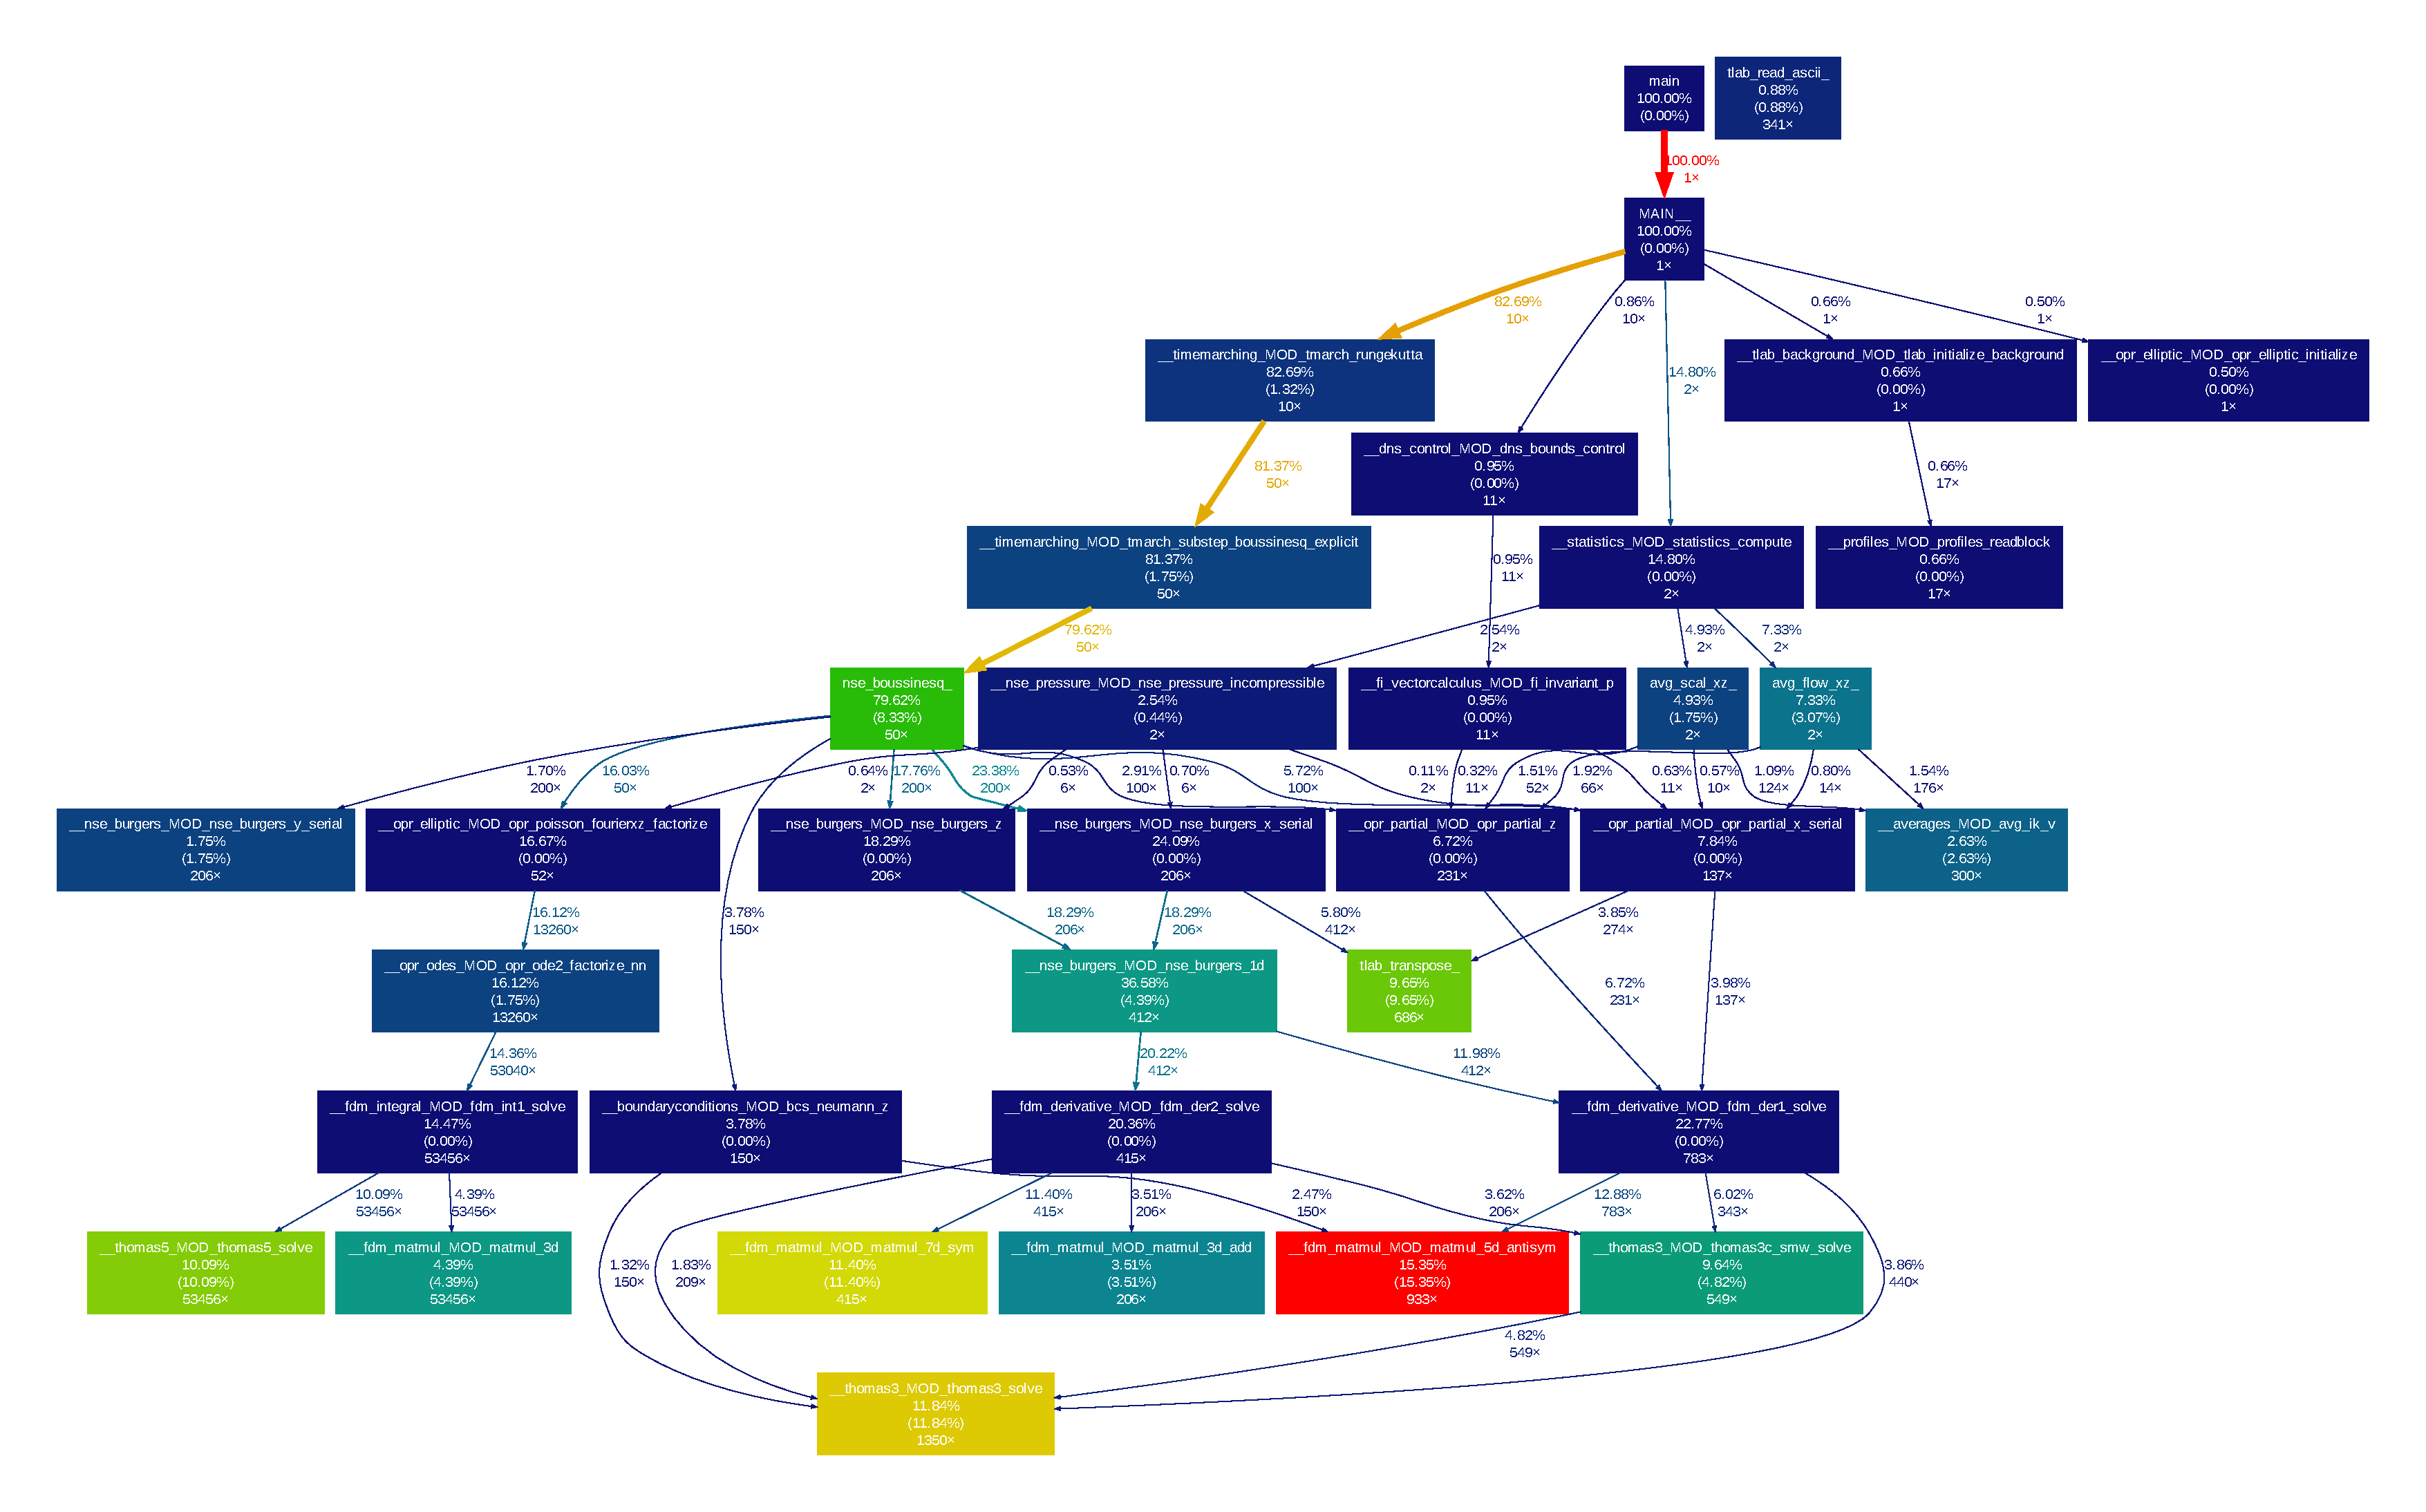
\includegraphics[clip,width=\textwidth]{fig-profiling08.pdf}
  \caption{Profiling diagram of \texttt{examples/Case08} running 10 iterations in serial mode. Profiling data obtained from \texttt{gfortran -pg} and processed with \texttt{gprof}, running the command \texttt{gprof path/to/your/executable | gprof2dot --color-nodes-by-selftime | dot -Tpdf -o output.pdf}.}
\end{figure}

\newpage

\begin{figure}[!h]
  \centering
  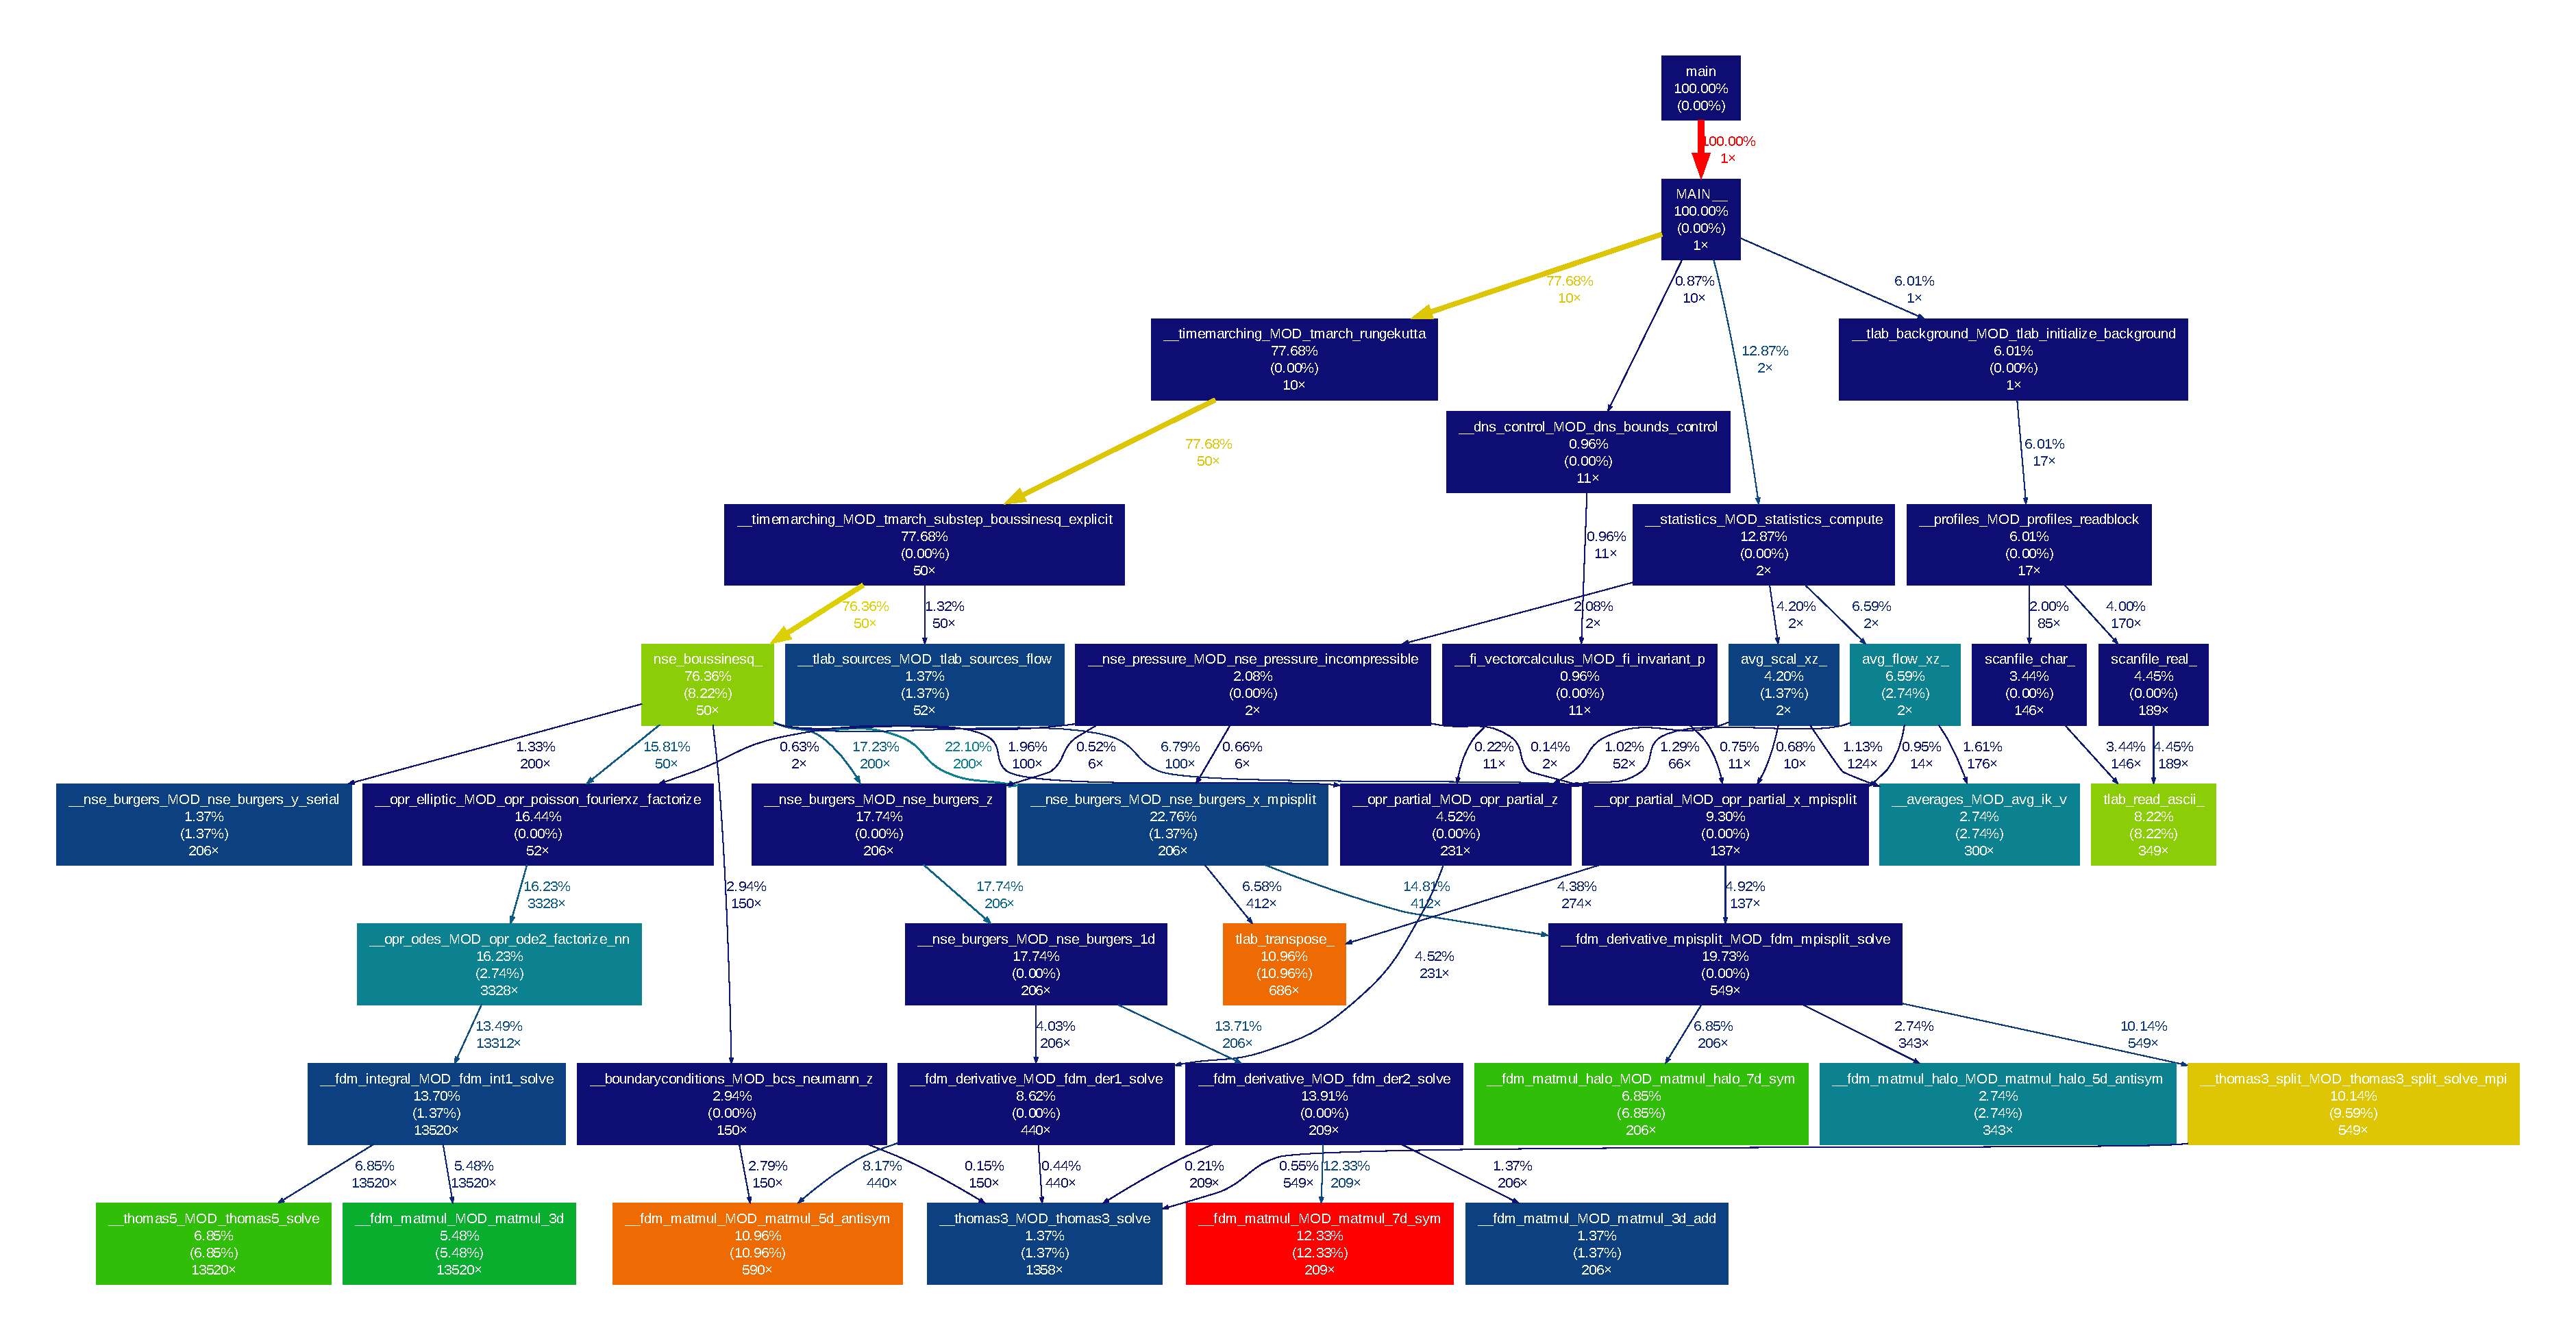
\includegraphics[clip,width=\textwidth]{fig-profiling08-mpi.pdf}
  \caption{Profiling diagram of \texttt{examples/Case08} running 10 iterations in parallel mode with 4 processors. Profiling data obtained from \texttt{gfortran -pg} and processed with \texttt{gprof}, running the command \texttt{gprof path/to/your/executable | gprof2dot --color-nodes-by-selftime | dot -Tpdf -o output.pdf}.}
\end{figure}

\newpage

\begin{figure}[!h]
  \centering
  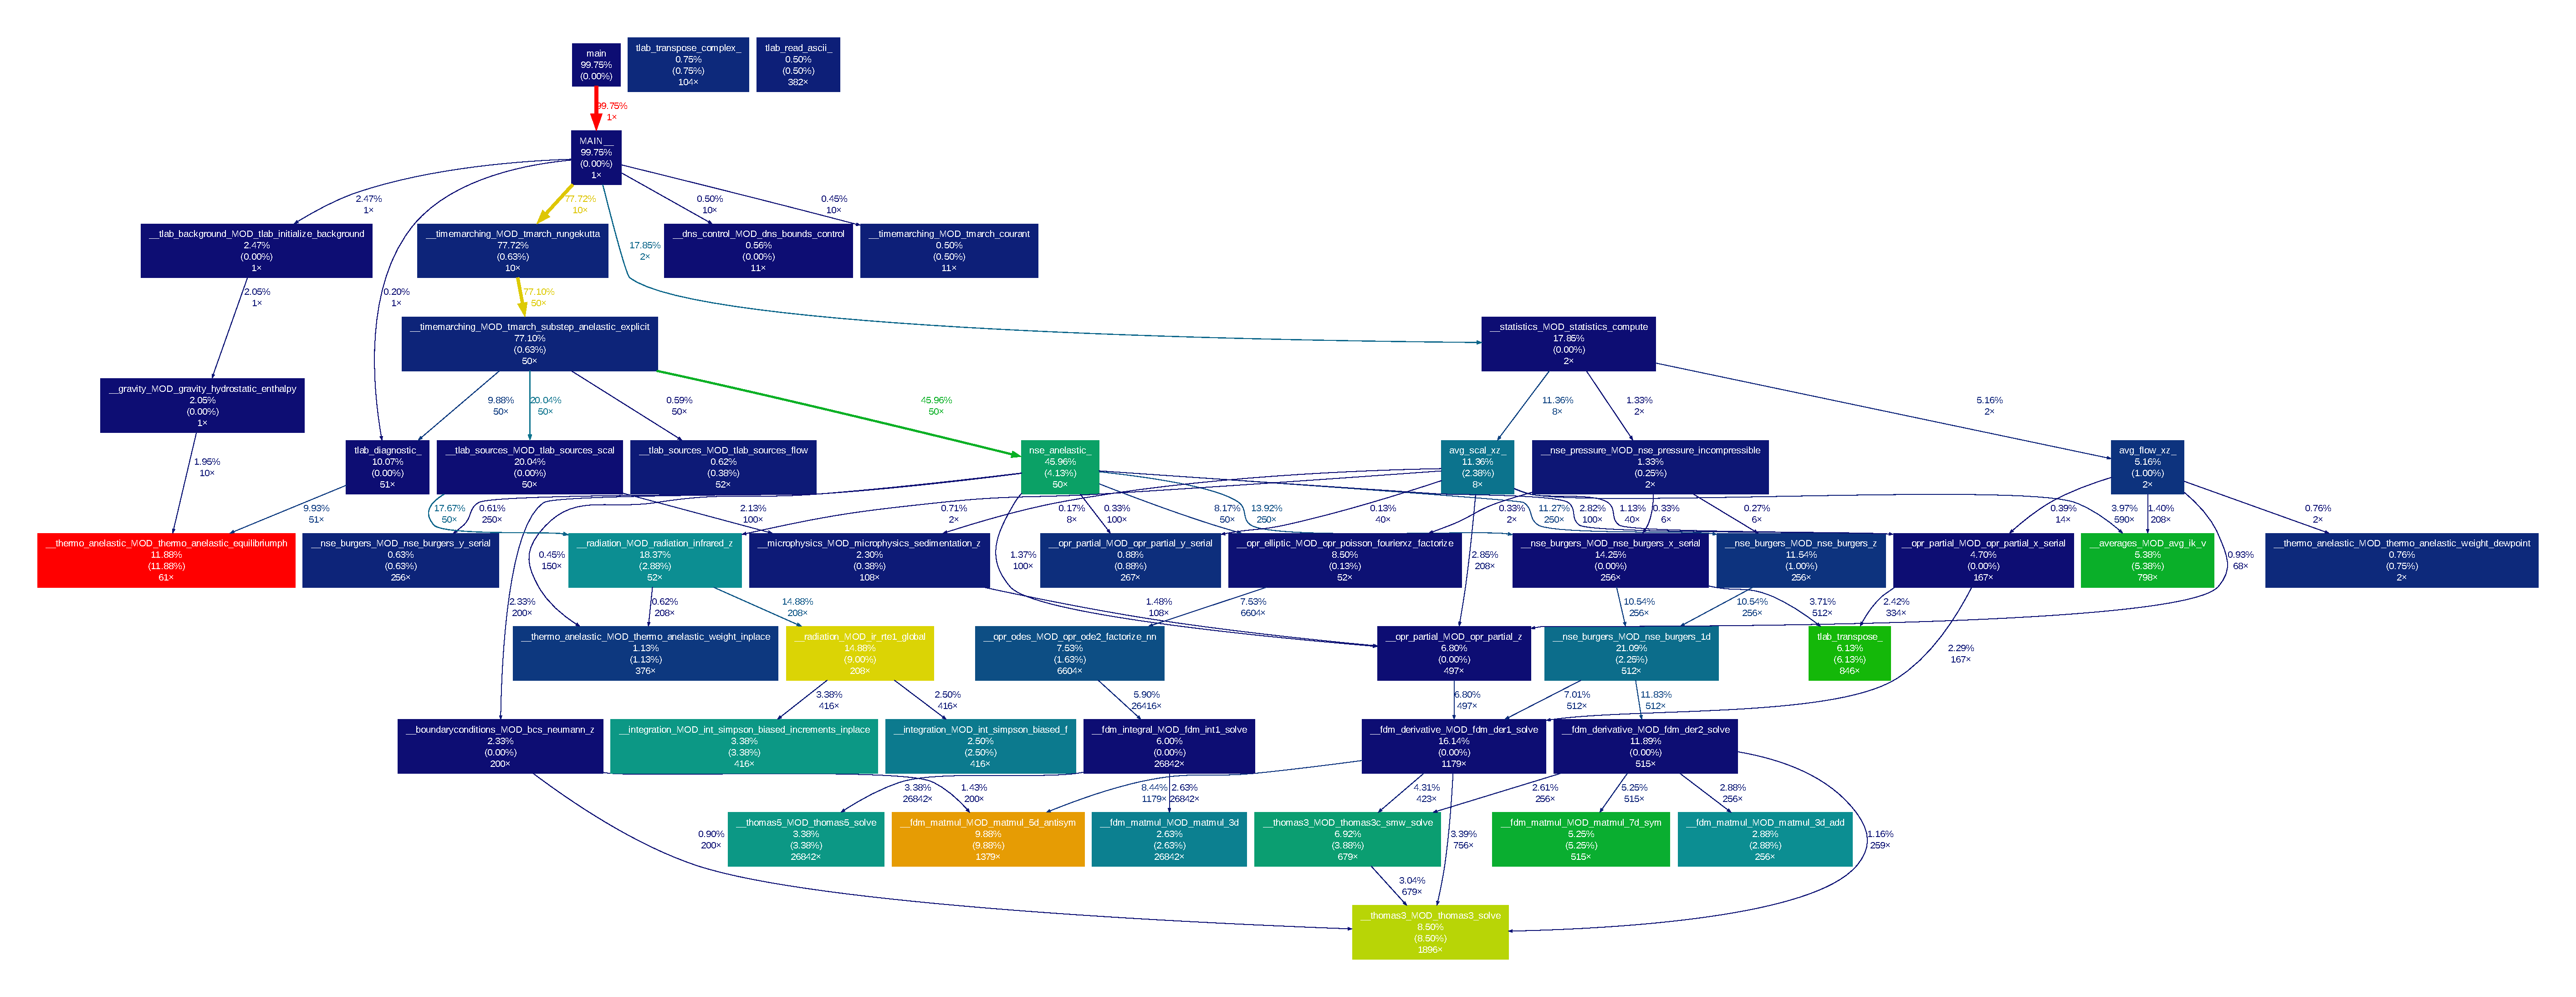
\includegraphics[clip,width=0.9\textheight,angle=90]{fig-profiling65.pdf}
  \caption{Profiling diagram of \texttt{examples/Case65} running 10 iterations in serial mode. Profiling data obtained from \texttt{gfortran -pg} and processed with \texttt{gprof}, running the command \texttt{gprof path/to/your/executable | gprof2dot --color-nodes-by-selftime | dot -Tpdf -o output.pdf}.}
\end{figure}

% \caption{Profiling diagram of modified \texttt{examples/Case44} (768 cube) running 25 iterations in parallel mode with 48 tasks (1 node on juwels).}
